
\providecommand{\sSet}{s\mathcal{S}et}%
\providecommand{\qcOne}{\mathbf{1}}%
\providecommand{\qcTwo}{\mathbf{2}}%

\section{切片与锥的等价}\label{sec:equivalence-of-slices-and-cones}

\cref{thm:natural-marking-complicial}与%
\cref{thm:isofibration-complicial-isofibration}也使我们得以最终证明 4.2 节
中概述的诸结果——这些结果如今从 D.2 节中所完成的组合工作出发即可轻易推得。
特别回顾\cref{prop:comparison-marked-homotopy-retract}：它表明增广单纯集的映射
\begin{equation*}
s^{n,m}\colon\Delta[n]\diamond\Delta[m]\longrightarrow\Delta[n]\star\Delta[m]
\qquad\in\sSet_{+}^{\Delta_{+}\times\Delta_{+}}
\end{equation*}
是一个带标记同伦收缩等价。据\cref{lem:marked-homotopy-equivalence-induces}，
我们现在知道：这类映射在映入诸\trQuasiCategory{}时诱导出\trEquivalence。

在本节中，我们利用这些观察验证：对任何增广单纯集 $X$ 与 $Y$，增广单纯集的
典范映射 $s^{X,Y}\colon X\diamond Y\to X\star Y$ 在映入诸\trQuasiCategory{}时
也诱导出\trEquivalence。为此，我们使用 C.5 节中发展的 Reedy 范畴论\trHomotopy{}%
理论。首先：

\begin{lemma}[\trLatchingMap]\label{lem:latching-maps-join-fat-join}
\emph{由
\begin{equation*}
F_{\diamond}^{n,m}\coloneqq\Delta[n]\diamond\Delta[m]
\qquad\text{与}\qquad
F_{\star}^{n,m}\coloneqq\Delta[n]\star\Delta[m]
\end{equation*}
所定义的诸\trDiagram{} $F_{\diamond},F_{\star}\in\sSet_{+}^{\Delta_{+}\times\Delta_{+}}$
的诸\trLatchingMap{}即为映射}
\begin{rveq}\label{eq:latching-maps}
\bigl(\partial\Delta[n]\hookrightarrow\Delta[n]\bigr)\mathbin{\hat{\diamond}}
\bigl(\partial\Delta[m]\hookrightarrow\Delta[m]\bigr)
\qquad\text{与}\qquad
\bigl(\partial\Delta[n]\hookrightarrow\Delta[n]\bigr)\mathbin{\hat{\star}}
\bigl(\partial\Delta[m]\hookrightarrow\Delta[m]\bigr)
\end{rveq}
\emph{二者皆为\trMonomorphism{}，从而 $F_{\diamond}$ 与 $F_{\star}$ 都是 Reedy
单态的}。
\end{lemma}

\begin{proof}
对任何一对增广单纯集 $X$ 与 $Y$，我们把它们的\textbf{外积}（external
product）$X\mathbin{\square}Y\in\mathcal{S}et^{\Delta_{+}^{\mathrm{op}}\times\Delta_{+}^{\mathrm{op}}}$
定义为把对象 $([n],[m])$ 送到集合 $X_{n}\times Y_{m}$ 的那个\trFunctor。特别地，
$([n],[m])$ 所表示的\trFunctor{}正是 $\Delta[n]\mathbin{\square}\Delta[m]$。我们
可以把一个外积 $X\mathbin{\square}Y$ 视为诸\trDiagram{} $F_{\diamond}$ 与
$F_{\star}$ 的一个权，并利用附录 A 中的\cref{def:weighted-limit-colimit-constructive}
以及\trJoin{}与\trFatJoin\trBifunctor{}的余连续性来计算诸\trWeightedColimit：
\begin{align*}
\operatorname{colim}_{X\mathbin{\square}Y}F_{\diamond}
&\cong\int\limits^{([n],[m])\in\Delta_{+}\times\Delta_{+}}
  \coprod_{X_{n}\times Y_{m}}\Delta[n]\diamond\Delta[m]\\
&\cong\Bigl(\int\limits^{[n]\in\Delta_{+}}\coprod_{X_{n}}\Delta[n]\Bigr)\diamond
  \Bigl(\int\limits^{[m]\in\Delta_{+}}\coprod_{Y_{m}}\Delta[m]\Bigr)\\
&\cong X\diamond Y
\end{align*}
类似地，$\operatorname{colim}_{X\mathbin{\square}Y}F_{\star}\cong X\star Y$。

据\cref{def:latching-matching-objects}，在对象 $([n],[m])\in\Delta_{+}\times\Delta_{+}$
处的\trLatchingMap，是由权之间的映射
\begin{equation*}
(\partial\Delta[n]\hookrightarrow\Delta[n])\mathbin{\square}
(\partial\Delta[m]\hookrightarrow\Delta[m])
\end{equation*}
所诱导的、\trWeightedColimit{}上的那个映射。由刚才给出的\trWeightedColimit{}计算可见，%
$F_{\diamond}$ 与 $F_{\star}$ 的诸\trLatchingMap{}正是 \eqref{eq:latching-maps} 的那些
映射。

尚须验证这些\trLatchingMap{}都是\trMonomorphism。经直接计算，
\begin{equation*}
(\partial\Delta[n]\hookrightarrow\Delta[n])\mathbin{\hat{\star}}
(\partial\Delta[m]\hookrightarrow\Delta[m])
\cong\partial\Delta[n+1+m]\hookrightarrow\Delta[n+1+m]\mbox{,}
\end{equation*}
它显然是一个\trMonomorphism，故 $F_{\star}$ 是 Reedy 单态的。

至于\trFatJoin{}的类似结果，首先注意到
\begin{equation*}
(\partial\Delta[-1]\hookrightarrow\Delta[-1])\mathbin{\hat{\diamond}}
(X\hookrightarrow Y)\cong(X\hookrightarrow Y)\mbox{,}
\end{equation*}
因为 $\partial\Delta[-1]$ 是\trInitial{}对象，而 $\Delta[-1]$ 是\trFatJoin{}的单位。
于是，只须考虑诸\trSimplex{}\trBoundary{}包含与 $n,m\ge 0$ 的\trLeibnizProduct；此时，
由于 $\partial\Delta[n]$ 与 $\Delta[n]$ 都是终增广的，\trFatJoin{}的公式得以化简。回顾
第 4 章中的\cref{def:fat-join}：对终增广单纯集 $X$ 与 $Y$ 以及 $n\ge 0$，
$(X\diamond Y)_{n}\cong X_{n}\sqcup\bigl(\coprod_{[n]\to[1]}X_{n}\times Y_{n}\bigr)\sqcup Y_{n}$。
于是我们看到：对终增广单纯集的任意\trMonomorphism{} $X\hookrightarrow Y$ 与
$U\hookrightarrow V$，方块
\begin{center}
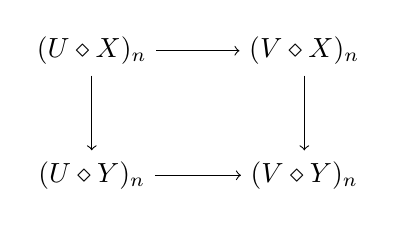
\begin{tikzpicture}[x=1.6em,y=1.5em]
  \node (tl) at (0,1.5) {$(U\diamond X)_{n}$};
  \node (tr) at (4.8,1.5) {$(V\diamond X)_{n}$};
  \node (bl) at (0,-1.5) {$(U\diamond Y)_{n}$};
  \node (br) at (4.8,-1.5) {$(V\diamond Y)_{n}$};
  \draw[->] (tl) -- (tr);
  \draw[->] (bl) -- (br);
  \draw[->] (0,0.9) -- (0,-0.9);
  \draw[->] (4.8,0.9) -- (4.8,-0.9);
  \node at (1.4,0) {$\scriptstyle\lrcorner$};
\end{tikzpicture}
\end{center}
是集合范畴中的一个\trPullback。对集合范畴中任何由诸\trMonomorphism{}构成的%
\trPullback{}方块，方块内部之\trPushout{}由其下方一条腿与右侧一条腿的联合像
构造而成：特别地，映射
$(U\diamond Y)_{n}\cup_{(U\diamond X)_{n}}(V\diamond X)_{n}\hookrightarrow(V\diamond Y)_{n}$
是一个\trMonomorphism。从而，终增广单纯集的两支\trMonomorphism{}的 Leibniz
\trFatJoin $(U\hookrightarrow V)\mathbin{\hat{\diamond}}(X\hookrightarrow Y)$ 是一个%
\trMonomorphism，特别地，$F_{\diamond}$ 的诸\trLatchingMap{}如所宣称地都是%
\trMonomorphism。
\end{proof}

回顾\cref{lem:fat-join-comparison}——从一对单纯集的\trFatJoin{}到这一对单纯集的\trJoin{}的
自然比较映射。我们现在得以证明第 4 章中的\cref{prop:join-vs-fat-join}。

\begin{proposition}\label{prop:fat-join-comparison-weak-equivalence}
\emph{对一切单纯集 $X$ 与 $Y$，自然映射 $s^{X,Y}\colon X\diamond Y\to X\star Y$
对每个\trQuasiCategory{} $A$ 都诱导出诸\trQuasiCategory{}之间的一个%
\trEquivalence}
$A^{X\star Y}\twoheadrightarrow A^{X\diamond Y}$\emph{。}
\end{proposition}

Lurie 在 \cite[4.2.1.2]{bib78} 中给出了本结果的另一个证明。

\begin{proof}
一次直接的验证表明：增广双单纯集
$X\mathbin{\square}Y\in\mathcal{S}et^{\Delta_{+}^{\mathrm{op}}\times\Delta_{+}^{\mathrm{op}}}$
的诸\trLatchingMap{}都是\trMonomorphism。\footnote{这由 $\Delta_{+}\times\Delta_{+}$ 是
一个\textbf{优雅 Reedy 范畴}（elegant Reedy category）这一事实得到：以该范畴为
标引的预层的每个元素都以唯一的方式是某个非退化元素的退化 \cite{bib16}，从而
一切预层都是 Reedy 单态的。}于是，据附录 C 中的%
\cref{cor:reedy-quillen-weighted-functors}，\trWeightedColimit{}函子
\begin{equation*}
\operatorname{colim}_{X\mathbin{\square}Y}-\colon
\sSet^{\Delta_{+}\times\Delta_{+}}\longrightarrow\sSet
\end{equation*}
是从 Joyal \trModelStructure{}的 Reedy 版本到单纯集上的 Joyal
\trModelStructure{}的一个左 Quillen 二函子。

据\cref{prop:comparison-marked-homotopy-retract}与%
\cref{lem:marked-homotopy-equivalence-induces}，诸分量
$s^{n,m}\colon\Delta[n]\diamond\Delta[m]\to\Delta[n]\star\Delta[m]$ 是 Joyal
\trModelStructure{}中的\trWeakEquivalence，因为后者恰被刻画为那些在映入任意%
\trQuasiCategory{}时诱导出\trEquivalence{}的映射。于是，%
\cref{prop:comparison-marked-homotopy-retract}与\cref{lem:latching-maps-join-fat-join}
建立起：自然变换 $s\colon F_{\diamond}\to F_{\star}$ 是
$\sSet_{+}^{\Delta_{+}\times\Delta_{+}}$ 中 Reedy \trCofibrant{}对象之间的一个%
\trPointwise{}\trWeakEquivalence。据附录 C 中的\cref{lem:quillen-preserves-we}，
\trWeightedColimit{}上诱导的映射 $s^{X,Y}\colon X\diamond Y\to X\star Y$ 便是 Joyal
\trModelStructure{}中的一个\trWeakEquivalence，而这恰好意味着：它对每个%
\trQuasiCategory{} $A$ 都诱导出诸\trQuasiCategory{}之间的一个\trEquivalence
$A^{X\star Y}\twoheadrightarrow A^{X\diamond Y}$，如所宣称。
\end{proof}

特别地，对任何\trQuasiCategory{} $A$，存在自然的\trEquivalence
$A^{\qcOne\star J}\twoheadrightarrow A^{\qcOne\diamond J}$ 与
$A^{J\star\qcOne}\twoheadrightarrow A^{J\diamond\qcOne}$，卧于 $A\times A^{J}$
之上。据第 4 章中的\cref{lem:fat-join-cones}，二者的余定义域沿拉回定义出%
\trDiagram{} $d\colon J\to A$ 之上或之下的诸锥\trQuasiCategory。然而，一如第 4
章中的\cref{war:slice-notation}所讨论的，二者的定义域并不能沿拉回给出
\cref{def:slices-of-simplicial-sets}的切片\trQuasiCategory{} $A_{/d}$ 与
${}^{d/}\!A$。尽管如此，我们可以利用\trJoin{}构造与\trFatJoin{}构造之间的这一%
\trEquivalence{}来证明 $A_{/d}$ 与 $\mathrm{Hom}_{A^{J}}(\Delta,d)$、%
${}^{d/}\!A$ 与 $\mathrm{Hom}_{A^{J}}(d,\Delta)$ 卧于 $A$ 之上相互等价，现在就
来做这件事。

\begin{proposition}\label{prop:slices-cones-equivalence}
\emph{对任何由单纯集 $J$ 标引、取值于\trQuasiCategory{} $A$ 的\trDiagram{}
$d\colon J\to A$，存在自然的\trEquivalence}
\begin{center}
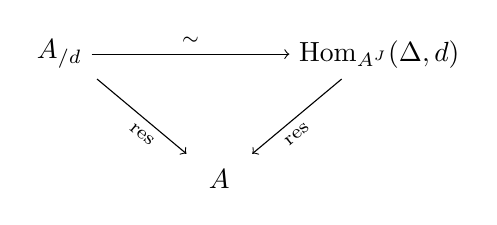
\begin{tikzpicture}[x=1.7em,y=1.5em]
  \node (l) at (0,1.5) {$A_{/d}$};
  \node (r) at (6.8,1.5) {$\mathrm{Hom}_{A^{J}}(\Delta,d)$};
  \node (b) at (3.4,-1.5) {$A$};
  \draw[->] (l) -- node[above]{$\scriptstyle\sim$} (r);
  \draw[->] (0.8,0.9) -- node[below,sloped,pos=0.6]{$\scriptstyle\mathrm{res}$} (2.7,-0.9);
  \draw[->] (6.0,0.9) -- node[below,sloped,pos=0.6]{$\scriptstyle\mathrm{res}$} (4.1,-0.9);
\end{tikzpicture}
\qquad
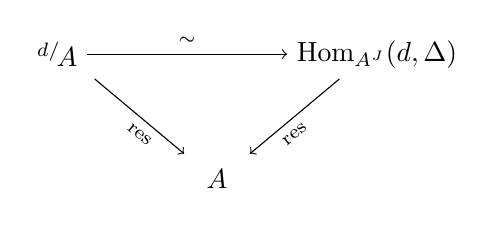
\begin{tikzpicture}[x=1.7em,y=1.5em]
  \node (l) at (0,1.5) {${}^{d/}\!A$};
  \node (r) at (6.8,1.5) {$\mathrm{Hom}_{A^{J}}(d,\Delta)$};
  \node (b) at (3.4,-1.5) {$A$};
  \draw[->] (l) -- node[above]{$\scriptstyle\sim$} (r);
  \draw[->] (0.8,0.9) -- node[below,sloped,pos=0.6]{$\scriptstyle\mathrm{res}$} (2.7,-0.9);
  \draw[->] (6.0,0.9) -- node[below,sloped,pos=0.6]{$\scriptstyle\mathrm{res}$} (4.1,-0.9);
\end{tikzpicture}
\end{center}
\emph{介于诸切片拟范畴与诸锥\trQuasiCategory{}之间}。
\end{proposition}

\begin{proof}
我们的证明再次动用 Reedy 范畴论。首先，回顾\cref{def:slices-of-simplicial-sets}
的\trAdjunction
\begin{center}
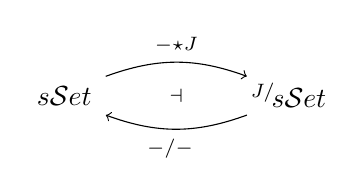
\begin{tikzpicture}[x=1.5em,y=1.4em]
  \node (s) at (0,0) {$\sSet$};
  \node (j) at (5.4,0) {${}^{J/}\!\sSet$};
  \draw[->] (1.0,0.5) to[bend left=20] node[above]{$\scriptstyle-\star J$} (4.4,0.5);
  \node at (2.7,0) {$\scriptstyle\dashv$};
  \draw[->] (4.4,-0.5) to[bend left=20] node[below]{$\scriptstyle-/-\;\;$} (1.0,-0.5);
\end{tikzpicture}
\end{center}
它给出这样一个对应：对单纯集 $I$ 与映射 $d\colon J\to A$，$J$ 之下的映射
$I\star J\to A$ 与单纯集的映射 $I\to A_{/d}$ 一一对应。\trFatJoin\trFunctor
$-\diamond J\colon\sSet\to{}^{J/}\!\sSet$ 的一个\trRightAdjoint{}可以类似地算
出。据第 4 章中的\cref{def:fat-join}的定义性\trPushout，上图所示的、$J$ 之下的
映射 $I\diamond J\to A$ 的数据经转置即为下图所示的数据
\begin{center}
\begin{tikzpicture}[x=1.6em,y=1.5em]
  \node (tl) at (0,1.7) {$(I\times J)\sqcup(I\times J)$};
  \node (tr) at (7.2,1.7) {$I\sqcup J$};
  \node (bl) at (0,-1.7) {$I\times\qcTwo\times J$};
  \node (bm) at (7.2,-1.7) {$I\diamond J$};
  \node (A) at (10.8,-1.7) {$A$};
  \draw[->] (tl) -- node[above]{$\scriptstyle\pi_{I}\sqcup\pi_{J}$} (tr);
  \draw[right hook->] (0,1.1) -- (0,-1.1);
  \draw[right hook->] (7.2,1.1) -- node[pos=0.45,right]{$\scriptstyle-\sqcup\mathrm{id}$} (7.2,-1.1);
  \draw[->] (bl) -- (bm);
  \draw[->,dashed] (bm) -- (A);
  \draw[->] (7.9,1.4) -- node[pos=0.4,right]{$\scriptstyle-\sqcup d$} (10.4,-1.4);
  \node at (6.3,-0.6) {$\scriptstyle\llcorner$};
  \begin{scope}[shift={(0.4,-6.0)}]
    \node (I) at (0,1.7) {$I$};
    \node (hom) at (4.6,1.7) {$\mathrm{Hom}_{A^{J}}(\Delta,d)$};
    \node (a2j) at (10.0,1.7) {$A^{\qcTwo\times J}$};
    \node (oa) at (4.6,-1.7) {$1\times A$};
    \node (ajaj) at (10.0,-1.7) {$A^{J}\times A^{J}$};
    \draw[->,dotted] (0.6,1.7) -- (2.9,1.7);
    \draw[->] (6.4,1.7) -- (8.3,1.7);
    \draw[->] (0.5,1.3) -- (3.3,-1.3);
    \draw[->] (4.6,1.1) -- (4.6,-1.1);
    \draw[->] (10.0,1.1) -- (10.0,-1.1);
    \draw[->] (oa) -- node[below]{$\scriptstyle d\times\Delta$} (ajaj);
    \node at (5.4,0.5) {$\scriptstyle\lrcorner$};
  \end{scope}
\end{tikzpicture}
\end{center}
于是我们看到，$-\diamond J$ 的\trRightAdjoint
\begin{center}
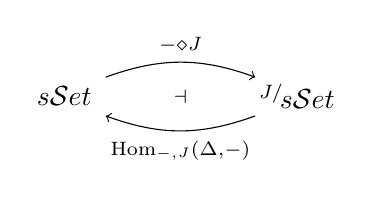
\begin{tikzpicture}[x=1.5em,y=1.4em]
  \node (s) at (0,0) {$\sSet$};
  \node (j) at (5.6,0) {${}^{J/}\!\sSet$};
  \draw[->] (1.0,0.5) to[bend left=20] node[above]{$\scriptstyle-\diamond J$} (4.6,0.5);
  \node at (2.8,0) {$\scriptstyle\dashv$};
  \draw[->] (4.6,-0.5) to[bend left=20] node[below]{$\scriptstyle\mathrm{Hom}_{-,J}(\Delta,-)$} (1.0,-0.5);
\end{tikzpicture}
\end{center}
在 $d\colon J\to A$ 处的值定义了 $d$ 之上的\trInfinityCategoryOfCones{}
$\mathrm{Hom}_{A^{J}}(\Delta,d)$。

\cref{lem:fat-join-comparison}的自然映射 $s^{X,Y}\colon X\diamond Y\to X\star Y$
定义一个自然变换
\begin{center}
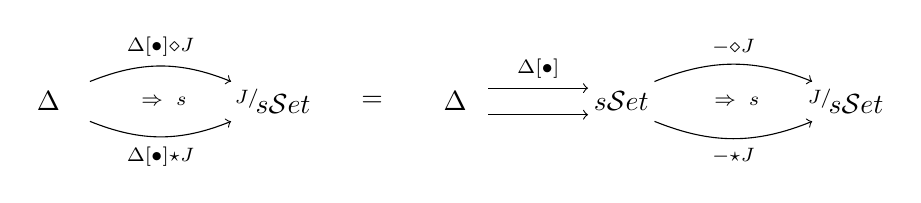
\begin{tikzpicture}[x=1.5em,y=1.6em]
  \node (d1) at (0,0) {$\Delta$};
  \node (j1) at (5.4,0) {${}^{J/}\!\sSet$};
  \draw[->] (1.0,0.45) to[bend left=22] node[above]{$\scriptstyle\Delta[\bullet]\diamond J$} (4.4,0.45);
  \draw[->] (1.0,-0.45) to[bend right=22] node[below]{$\scriptstyle\Delta[\bullet]\star J$} (4.4,-0.45);
  \node at (2.5,0) {$\scriptstyle\Rightarrow$};
  \node at (3.2,0) {$\scriptstyle s$};
  \node at (7.8,0) {$=$};
  \begin{scope}[shift={(9.8,0)}]
    \node (d2) at (0,0) {$\Delta$};
    \node (ss) at (4.0,0) {$\sSet$};
    \node (j2) at (9.4,0) {${}^{J/}\!\sSet$};
    \draw[->] (0.8,0.3) -- node[above]{$\scriptstyle\Delta[\bullet]$} (3.2,0.3);
    \draw[->] (0.8,-0.3) -- (3.2,-0.3);
    \draw[->] (4.8,0.45) to[bend left=22] node[above]{$\scriptstyle-\diamond J$} (8.6,0.45);
    \draw[->] (4.8,-0.45) to[bend right=22] node[below]{$\scriptstyle-\star J$} (8.6,-0.45);
    \node at (6.5,0) {$\scriptstyle\Rightarrow$};
    \node at (7.2,0) {$\scriptstyle s$};
  \end{scope}
\end{tikzpicture}
\end{center}
据\cref{prop:fat-join-comparison-weak-equivalence}，它是（切片的）Joyal
\trModelStructure{}中的一个\trPointwise{}\trWeakEquivalence。注意，经伴随性，
$\mathrm{Hom}_{A^{J}}(\Delta,d)$ 同构于在 ${}^{J/}\!\sSet$ 中从余单纯对象
$\Delta[\bullet]\diamond J$ 映到 $d\colon J\to A$ 所定义的单纯集，而 $A_{/d}$
同构于在 ${}^{J/}\!\sSet$ 中从余单纯对象 $\Delta[\bullet]\star J$ 映到
$d\colon J\to A$ 所定义的单纯集。特别地，自然变换 $s$ 的\trMate{}定义一个自然
比较映射 $\hat{s}\colon A_{/d}\to\mathrm{Hom}_{A^{J}}(\Delta,d)$。此外，由于
$s^{\Delta[\bullet],\varnothing}$ 是恒同，这一自然比较映射卧于 $A$ 之上。又请
注意：余单纯对象 $\Delta[\bullet]\diamond J$ 与 $\Delta[\bullet]\star J$ 皆不
可增广，从而据附录 C 中的\cref{lem:unaugmentable-cosimplicial}是 Reedy
\trCofibrant{}的。

范畴 ${}^{J/}\!\sSet$ 中的 hom 二函子定义一个二函子
\begin{equation*}
\bigl(({}^{J/}\!\sSet)^{\Delta}\bigr)^{\mathrm{op}}\times{}^{J/}\!\sSet
\xrightarrow{\ \mathrm{hom}\ }
\mathcal{S}et^{\Delta^{\mathrm{op}}}=:\sSet
\end{equation*}
\begin{rveq}\label{eq:hom-bifunctor-square}
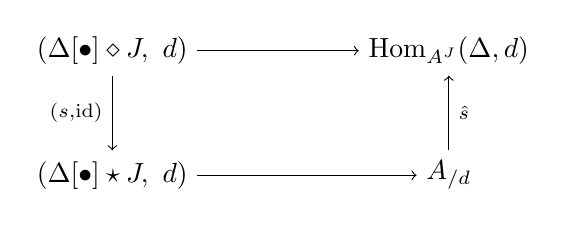
\begin{tikzpicture}[x=1.6em,y=1.5em]
  \node (tl) at (0,1.5) {$(\Delta[\bullet]\diamond J,\ d)$};
  \node (tr) at (7.6,1.5) {$\mathrm{Hom}_{A^{J}}(\Delta,d)$};
  \node (bl) at (0,-1.5) {$(\Delta[\bullet]\star J,\ d)$};
  \node (br) at (7.6,-1.5) {$A_{/d}$};
  \draw[->] (tl) -- (tr);
  \draw[->] (bl) -- (br);
  \draw[->] (0,0.9) -- node[left]{$\scriptstyle(s,\mathrm{id})$} (0,-0.9);
  \draw[->] (7.6,-0.9) -- node[right]{$\scriptstyle\hat{s}$} (7.6,0.9);
\end{tikzpicture}
\end{rveq}
它把映射 $s$ 与对象 $d\colon J\to A$ 送到卧于 $A$ 之上的映射
$\hat{s}\colon A_{/d}\to\mathrm{Hom}_{A^{J}}(\Delta,d)$。

据附录 C 中的\cref{lem:set-tensor-leibniz}，任何\trModelCategory{}——诸如
${}^{J/}\!\sSet$——的 hom 二函子都是右 Quillen 二函子，此处相对于附录 C 中的
\cref{ex:set-model-category}在 $\mathcal{S}et$ 上给出的那个\trModelStructure
而言，且两个\trWeakFactorizationSystem{}均取为（\trMonomorphism，%
\trEpimorphism）。现在，由于 $\Delta$ 是一个 Reedy 范畴，附录 C 中的%
\cref{thm:functor-tensor-product-leibniz}告诉我们：二函子
\eqref{eq:hom-bifunctor-square} 再次是右 Quillen 的，这次相对于
$({}^{J/}\!\sSet)^{\Delta}$ 上的 Reedy \trModelStructure{}与 $\mathcal{S}et^{\Delta^{\mathrm{op}}}$
上两个\trWeakFactorizationSystem{}均取为（Reedy \trMonomorphism，Reedy
\trEpimorphism）的那个\trModelStructure。据附录 C 中的%
\cref{lem:mono-epi-reedy-sset}，后一\trWeakFactorizationSystem{}与 $\sSet$ 上
熟知的（\trMonomorphism，\trTrivialFibration）\trWeakFactorizationSystem{}相
重合。

特别地，这一二函子把其第一变量中的一支 Reedy 平凡余纤维化与其第二变量中的
一个纤维性对象 $d\colon J\to A$ 载为单纯集的一支\trTrivialFibration。据 Ken
Brown 的引理（附录 C 中的\cref{lem:ken-brown}），由此得到：%
\eqref{eq:hom-bifunctor-square} 把 Reedy \trCofibrant{}对象之间的一个%
\trPointwise{}\trWeakEquivalence{}载为卧于 $A$ 之上的诸\trQuasiCategory{}间的
一个\trFiberedEquivalence，这就证明了 $\hat{s}$ 定义了所宣称的拟范畴间纤维化
等价。
\end{proof}

在 $J=\qcOne$ 的情形，图表 $\alpha\colon\qcOne\to A$ 定义\trQuasiCategory{} $A$
的一个\trElement，我们便得到以不同概念表述的同一结果。

\begin{corollary}\label{cor:slice-cone-point}
\emph{对\trQuasiCategory{} $A$ 的任何\trElement{} $\alpha\colon\qcOne\to A$，
存在\trCanonical{}\trEquivalence}
$A_{/\alpha}\twoheadrightarrow\mathrm{Hom}_{A}(A,\alpha)$ \emph{与}
${}^{\alpha/}\!A\twoheadrightarrow\mathrm{Hom}_{A}(\alpha,A)$\emph{，二者均卧于
$A$ 之上}。
\end{corollary}

\begin{proof}
当 $J=\qcOne$ 时，\cref{prop:slices-cones-equivalence}中出现的%
\trConstantFunctor{} $\Delta\colon A\to A^{\qcOne}$ 归结为 $A$ 上的恒同函子。
\end{proof}

\subsection*{练习}

\begin{exercise}\label{ex:lurie-mapping-spaces}
在 \cite[\S1.2.2]{bib78} 中，Lurie 用如下的\trPullback{}定义了\trQuasiCategory{}
$A$ 的一对\trElement{} $x$ 与 $y$ 之间的右映射空间与左映射空间：
\begin{center}
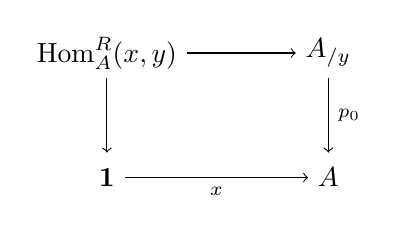
\begin{tikzpicture}[x=1.6em,y=1.5em]
  \node (h) at (0,1.5) {$\mathrm{Hom}_{A}^{R}(x,y)$};
  \node (a) at (5.0,1.5) {$A_{/y}$};
  \node (p) at (0,-1.5) {$\qcOne$};
  \node (A) at (5.0,-1.5) {$A$};
  \draw[->] (h) -- (a);
  \draw[->] (p) -- node[below]{$\scriptstyle x$} (A);
  \draw[->] (0,0.9) -- (0,-0.9);
  \draw[->] (5.0,0.9) -- node[right]{$\scriptstyle p_{0}$} (5.0,-0.9);
  \node at (1.4,0) {$\scriptstyle\lrcorner$};
\end{tikzpicture}
\qquad
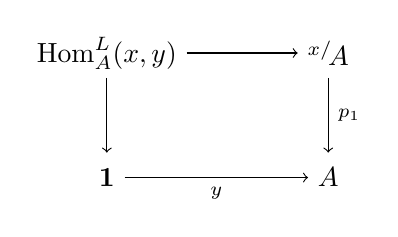
\begin{tikzpicture}[x=1.6em,y=1.5em]
  \node (h) at (0,1.5) {$\mathrm{Hom}_{A}^{L}(x,y)$};
  \node (a) at (5.0,1.5) {${}^{x/}\!A$};
  \node (p) at (0,-1.5) {$\qcOne$};
  \node (A) at (5.0,-1.5) {$A$};
  \draw[->] (h) -- (a);
  \draw[->] (p) -- node[below]{$\scriptstyle y$} (A);
  \draw[->] (0,0.9) -- (0,-0.9);
  \draw[->] (5.0,0.9) -- node[right]{$\scriptstyle p_{1}$} (5.0,-0.9);
  \node at (1.4,0) {$\scriptstyle\lrcorner$};
\end{tikzpicture}
\end{center}
证明：这些单纯集都是\trKanComplex，而且它们等价于第 3 章中的%
\cref{def:mapping-space}的\trMappingSpace：
\begin{equation*}
\mathrm{Hom}_{A}^{R}(x,y)\simeq\mathrm{Hom}_{A}(x,y)\simeq
\mathrm{Hom}_{A}^{L}(x,y)\mbox{.}
\end{equation*}
\end{exercise}

